\documentclass[11pt,a4paper]{article}
\usepackage[hyperref]{acl2017}
\usepackage{times}
\usepackage{latexsym}

\usepackage{url}
\usepackage{booktabs}
\usepackage{graphicx}

%\aclfinalcopy % Uncomment this line for the final submission
%\def\aclpaperid{***} %  Enter the acl Paper ID here

%\setlength\titlebox{5cm}
% You can expand the titlebox if you need extra space
% to show all the authors. Please do not make the titlebox
% smaller than 5cm (the original size); we will check this
% in the camera-ready version and ask you to change it back.

\newcommand\BibTeX{B{\sc ib}\TeX}

\title{Toward a Comparable Corpora of Latvian, Russian and English Tweets}

\author{First Author \\
  Affiliation / Address line 1 \\
  Affiliation / Address line 2 \\
  Affiliation / Address line 3 \\
  {\tt email@domain} \\\And
  Second Author \\
  Affiliation / Address line 1 \\
  Affiliation / Address line 2 \\
  Affiliation / Address line 3 \\
  {\tt email@domain} \\}

\date{}

\begin{document}
\maketitle
\begin{abstract}
\end{abstract}

\citet{milajevs-griffiths:2016:RepEval}

\section{Introduction}
\label{sec:introduction}



\section{Dataset construction}
\label{sec:construction}

The initial set of tweets was retrieved using the \texttt{POST status/filter} endpoint of the Twitter Streaming API.\footnote{\url{https://dev.twitter.com/streaming/reference/post/statuses/filter}} The collected tweets had to be geo-located and had to originate from the area of Riga, the capital of Latvia.\footnotemark{}

\footnotetext{The \texttt{locations} parameter was set to \texttt{23.9325829, 56.8570671, 24.3247299, 57.0859184}}

251\,083 tweets were collected from the period from the 1st of November 2016 to the 31st of March 2017. On April 14th 2017, the collection was rehydrated by querying the Twitter API with the collected tweet IDs to get rid of the deleted tweets. In addition, the tweets that originated retweets were included to the collection: the JSON representation of a retweet includes the original tweet, which we extracted and added to the collection. Rehydrated and expanded collection resulted to 220\,883 tweets. Table~\ref{tab:tweet-counts} summarises the number of collected tweets. 

\begin{table}[h]
  \centering
  \begin{tabular}{lrr}
    \toprule
    Collection & Tweet count \\
    \midrule
    Initial    & 222\,177    \\
    Rehydrated & 220\,883    \\
    Final      & 136\,067    \\
    \bottomrule
  \end{tabular}
  \caption{Tweet counts.}
  \label{tab:tweet-counts}
\end{table}

Further analysis of the extended rehydrated collection showed that there are 23115 (10.5\%) tweets that originated from the user check-ins with Swarm\footnote{\url{https://www.swarmapp.com/}} on Foursquare.\footnote{\url{https://foursquare.com/}} This motivated additional filtering of the rehydrated collection, as ``check-in tweets'' most of the time follow a predefined template and thus do not reflect real language use. 

\begin{table}[th]
  \small
  \centering
  \begin{tabular}{lrr}
    \toprule
    Client & Tweet count & Share \% \\
    \midrule
    Twitter Web Client     & 93\,705 &    42.4\% \\
    Twitter for iPhone     & 47\,721 &    21.6\% \\
    Twitter for Android    & 34\,277 &    15.5\% \\
    Foursquare$^*$             & 23\,115 &    10.5\% \\
    Instagram$^*$               & 13\,196 &     5.0\% \\
    Twitter for iPad       & 2\,420  &     1.1\% \\
    Endomondo$^*$               & 1\,611  &     0.7\% \\
    Tweetbot of iOS        & 1\,411  &     0.6\% \\
    World Cities$^*$            & 1\,361  &     0.6\% \\
    Linkis$^*$                  &  660  &     0.3\% \\
    \bottomrule
  \end{tabular}
  \caption{The top ten of Twitter clients in the rehydrated collection. $^*$Clients
    that are not included in the final collection as they do not exhibit
    linguistic value.}
  \label{tab:client-counts}
\end{table}

Table~\ref{tab:client-counts} shows the top ten most popular clients in the rehydrated collection. Together with the tweets originated from Foursquare, tweets from Instagram, an image sharing service), and Endomondo, a workout tracking service, were removed. Tweets written using the ``Word Cities'' client that posts weather reports and the Linkis client, a promotion website, were also removed.

The final collection resulted into 136\,067 tweets which are in Latvian, Russian or English and created after 1st of November 2016. The language of a tweet is provided by the corresponding field in the tweet JSON representation.


\begin{figure*}[t]
\centering
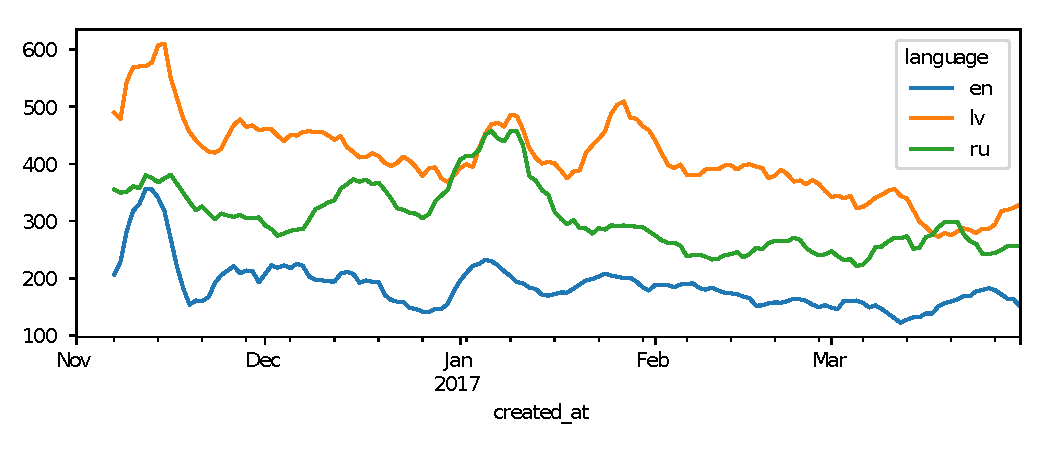
\includegraphics[width=\textwidth]{supplement/figures/timeline.pdf}
\caption{Tweet counts per day per language. The values are averaged over a week
  window at the right edge.}
\label{fig:timeline}
\end{figure*}

\section{Quantitative analysis}
\label{sec:quantitative}

Out of 136\,067 tweets that constitute the final collection, 45.5\% are in Latvian, 33.9\% are in Russian and 20.7\% are in English, see Table~\ref{tab:language-counts} for tweet counts. The ratio between the Latvian and Russian tweets is roughly the same as the proportion of ethnic Latvians and Russians in Riga, which is 46.2\% to 37.7\%.\footnote{\url{https://en.wikipedia.org/wiki/Riga}}

\begin{table}[ht]
  \centering
  \small
  \begin{tabular}{lrrr}
    \toprule
    Language & Tweet count & Share \% & Avg. token count \\
    \midrule
    Latvian     & 61\,869  & 45.4\% & 15 \\
    Russian     & 46\,070  & 33.9\% & 11 \\
    English     & 28\,128  & 20.7\% & 14 \\
    \bottomrule
  \end{tabular}
  \caption{Language distribution in the final collection.}
  \label{tab:language-counts}
\end{table}

Figure~\ref{fig:timeline} shows the bandwidth of tweets in time for all three languages. There are several peaks in Twitter usage.

\paragraph{Mid November}

18 November is the Proclamation Day of the Republic of Latvia. Numerous events take place across the country including torchlight processions and fireworks. The volume of tweets peaks in all three languages, thought the peak in Russian is less significant than in Latvian and English.

\paragraph{Mid December}

There is higher amount of Russian tweets, but Latvian and English tweet volume stays constant.

\paragraph{Early January}

There is a lot of activity during the New Year celebration for all three languages. Russian tweets peak the most almost reaching the same number of tweets as tweets in Latvian.

\paragraph{Late January}

In late January, the number of Latvian tweets increases, while for other languages it stays the same.

\paragraph{Mid March}

There is a general decline in Twitter usage for Latvian and English, but not for Russian, when for a short period of time there are more Russian tweets posted than Latvian.

\bibliography{references,dmilajevs_publications}
\bibliographystyle{acl_natbib}

\end{document}
